\chapter[Solução]{Solução}
A solução criada para resolver o problema de perda de conhecimento foi chamada de Repositório de Conhecimento. É uma solução de software criada a partir da ferramenta Bizagi Studio que visa automatizar esta pequena parte do processo de negócio da empresa para solucionar o problema especificado. 
Na solução é possível cadastrar e pesquisar problemas e soluções dadas pelos integrantes da equipe. Foi feita uma análise prévia de requisitos na qual muitos requisitos foram levantados junto ao cliente, no entanto, por motivos de tempo, somente algumas features foram priorizadas. 
As features priorizadas podem ser vistas no Capítulo 2 deste documento, onde encontra-se a rastreabilidade desde Temas de Investimento elicitados até as Histórias de Usuários detalhadas usando-se a técnica do 3C.

\begin{figure}[H]
\centering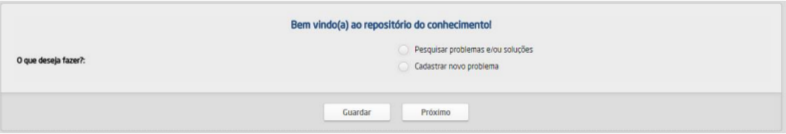
\includegraphics[scale=0.5]{figuras/paginaInicialSolucao.png}
\caption{\textit{Página inicial da solução}}
\end{figure}

Esta é a página inicial da solução onde o usuário tem a opção de pesquisar por problemas e/ou soluções, selecionando a opção desejada e o botão Próximo.

\begin{figure}[H]
\centering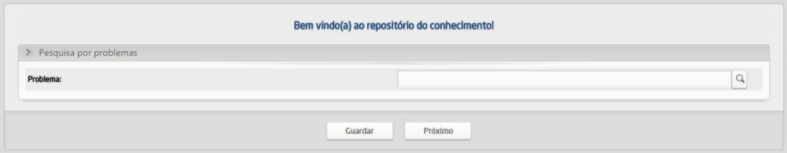
\includegraphics[scale=0.5]{figuras/pesquisaDeProblemas.png}
\caption{\textit{Pesquisa de problemas}}
\end{figure}

Ao escolher a opção de pesquisa de problemas e/ou soluções, o usuário é redirecionado para esta tela, onde clicando na lupa à esquerda do campo de Problema ele poderá fazer a busca desejada. 

\begin{figure}[H]
\centering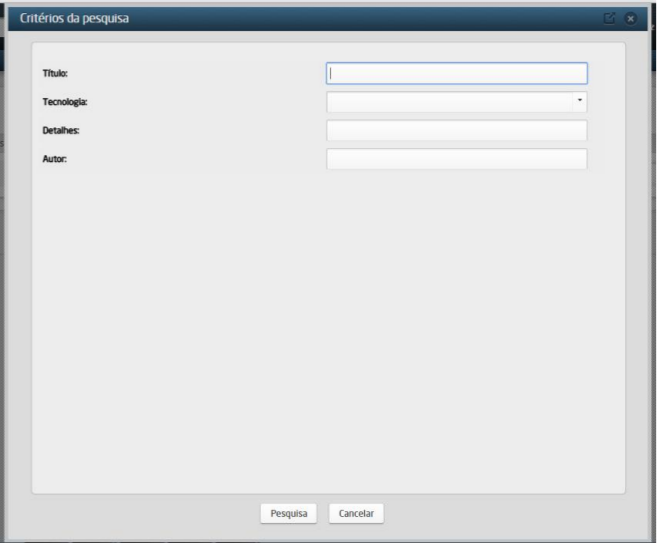
\includegraphics[scale=0.5]{figuras/buscaProblema.png}
\caption{\textit{Busca de problema por filtro}}
\end{figure}

O usuário poderá buscar problema através destes 4 filtros (utilizando um deles ou mais de um): título do problema, tecnologia relacionada a ele, detalhes do problema, autor do problema registrado. Em seguida, ele seleciona o botão Pesquisar. 

\begin{figure}[H]
\centering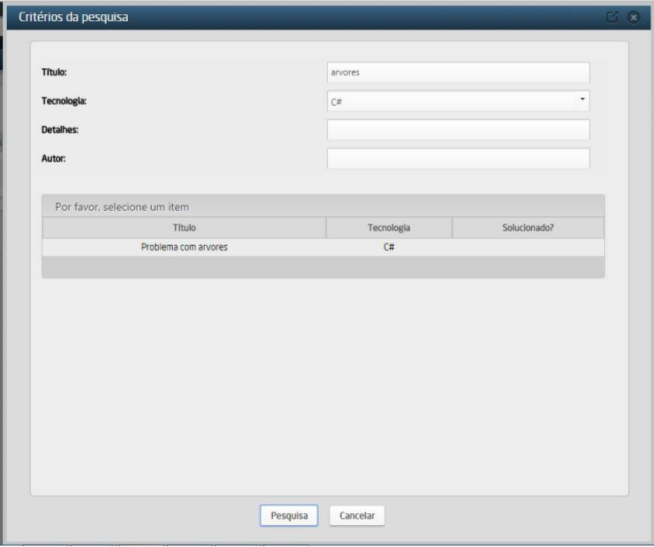
\includegraphics[scale=0.5]{figuras/resultadoBuscaProblema.png}
\caption{\textit{Resultado da busca por problema}}
\end{figure}

Pesquisando pelo título do problema “árvores” utilizando tecnologia “C\#”, são mostradas as soluções, que são clicáveis para visualizar soluções já cadastradas para aquele problema.

\begin{figure}[H]
\centering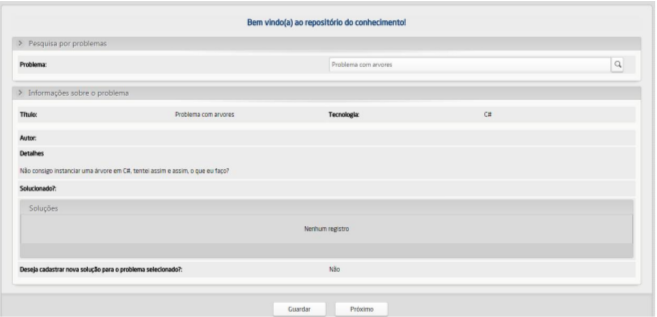
\includegraphics[scale=0.5]{figuras/selecaoProblemaSolucoes.png}
\caption{\textit{Seleção do problema para visualizar soluções}}
\end{figure}